\documentclass{standalone}
\usepackage{tikz}
\usetikzlibrary{patterns, positioning}

\begin{document}
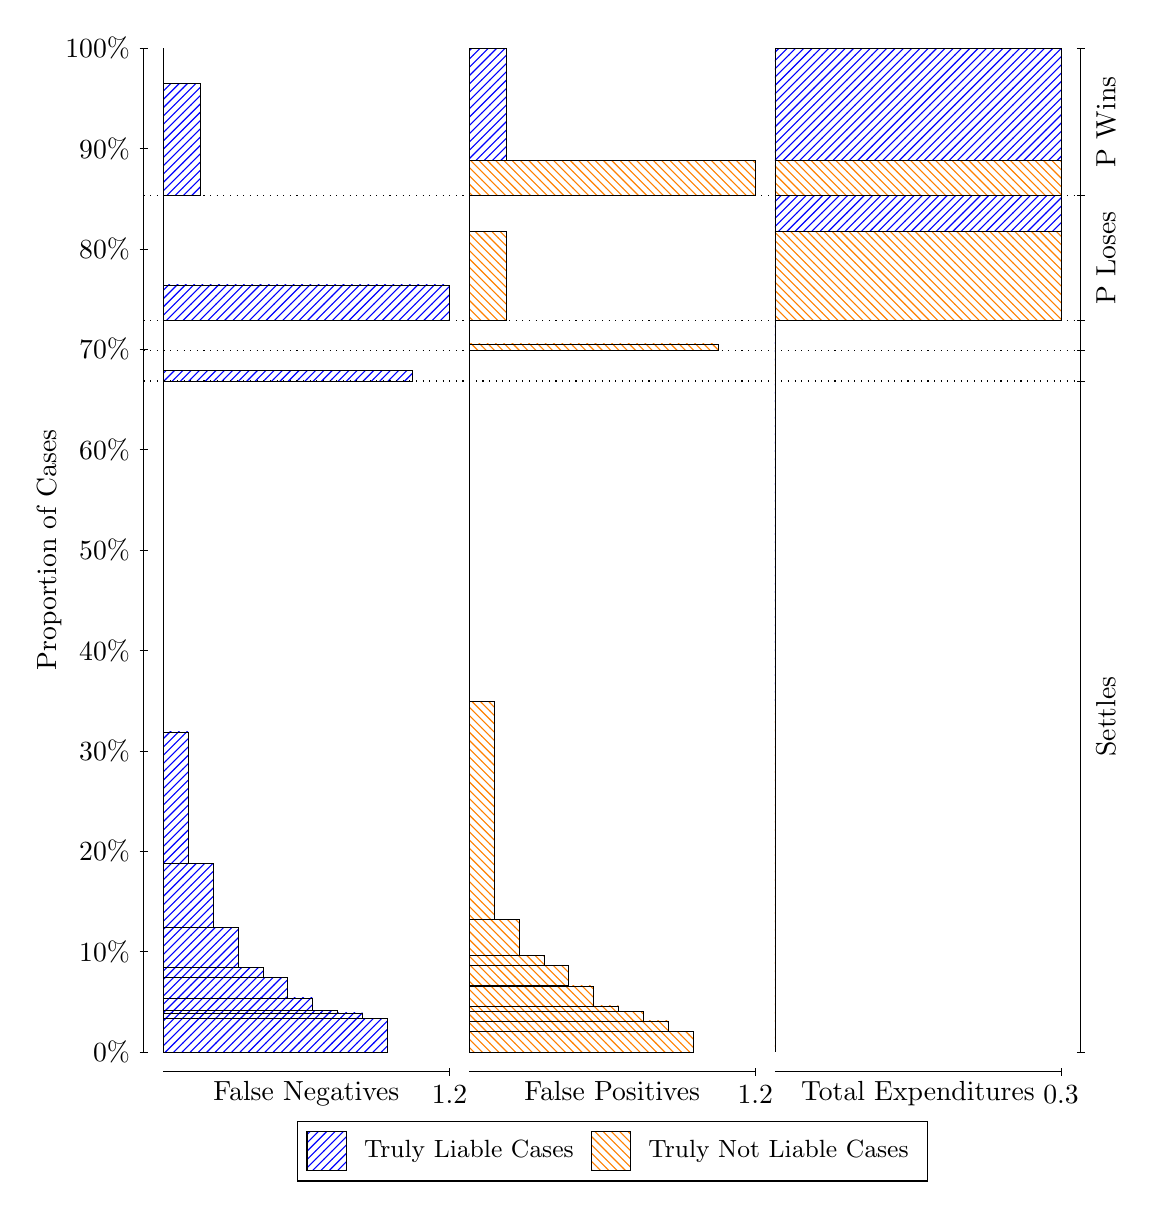
\begin{tikzpicture}
\draw[black, very thin] (1.5,1.75) -- (1.5,14.5);
\node[rotate=90, anchor=center] at (0.3, 8.125) {Proportion of Cases};
\draw[black, very thin] (1.45,1.75) -- (1.55,1.75);
\node[anchor=east] at (1.45, 1.75) {0\%};
\draw[black, very thin] (1.45,3.025) -- (1.55,3.025);
\node[anchor=east] at (1.45, 3.025) {10\%};
\draw[black, very thin] (1.45,4.3) -- (1.55,4.3);
\node[anchor=east] at (1.45, 4.3) {20\%};
\draw[black, very thin] (1.45,5.575) -- (1.55,5.575);
\node[anchor=east] at (1.45, 5.575) {30\%};
\draw[black, very thin] (1.45,6.85) -- (1.55,6.85);
\node[anchor=east] at (1.45, 6.85) {40\%};
\draw[black, very thin] (1.45,8.125) -- (1.55,8.125);
\node[anchor=east] at (1.45, 8.125) {50\%};
\draw[black, very thin] (1.45,9.4) -- (1.55,9.4);
\node[anchor=east] at (1.45, 9.4) {60\%};
\draw[black, very thin] (1.45,10.675) -- (1.55,10.675);
\node[anchor=east] at (1.45, 10.675) {70\%};
\draw[black, very thin] (1.45,11.95) -- (1.55,11.95);
\node[anchor=east] at (1.45, 11.95) {80\%};
\draw[black, very thin] (1.45,13.225) -- (1.55,13.225);
\node[anchor=east] at (1.45, 13.225) {90\%};
\draw[black, very thin] (1.45,14.5) -- (1.55,14.5);
\node[anchor=east] at (1.45, 14.5) {100\%};

\draw[black, very thin] (13.4,1.75) -- (13.4,14.5);
\draw[black, very thin] (13.35,1.75) -- (13.45,1.75);
\node[anchor=west] at (13.35, 1.75) {};
\draw[black, very thin] (13.35,10.271) -- (13.45,10.271);
\node[anchor=west] at (13.35, 10.271) {};
\draw[black, very thin] (13.35,10.662) -- (13.45,10.662);
\node[anchor=west] at (13.35, 10.662) {};
\draw[black, very thin] (13.35,11.041) -- (13.45,11.041);
\node[anchor=west] at (13.35, 11.041) {};
\draw[black, very thin] (13.35,12.626) -- (13.45,12.626);
\node[anchor=west] at (13.35, 12.626) {};
\draw[black, very thin] (13.35,14.5) -- (13.45,14.5);
\node[anchor=west] at (13.35, 14.5) {};

\draw[black, very thin, pattern color=blue, pattern=north east lines] (1.75,1.75) rectangle (4.5935,2.1764);
\draw[black, very thin, pattern color=blue, pattern=north east lines] (1.75,2.1764) rectangle (4.2775,2.2462);
\draw[black, very thin, pattern color=blue, pattern=north east lines] (1.75,2.2462) rectangle (3.9616,2.2828);
\draw[black, very thin, pattern color=blue, pattern=north east lines] (1.75,2.2828) rectangle (3.6457,2.4308);
\draw[black, very thin, pattern color=blue, pattern=north east lines] (1.75,2.4308) rectangle (3.6457,2.4371);
\draw[black, very thin, pattern color=blue, pattern=north east lines] (1.75,2.4371) rectangle (3.3297,2.6943);
\draw[black, very thin, pattern color=blue, pattern=north east lines] (1.75,2.6943) rectangle (3.0138,2.8235);
\draw[black, very thin, pattern color=blue, pattern=north east lines] (1.75,2.8235) rectangle (2.6978,3.3301);
\draw[black, very thin, pattern color=blue, pattern=north east lines] (1.75,3.3301) rectangle (2.3819,4.1459);
\draw[black, very thin, pattern color=blue, pattern=north east lines] (1.75,4.1459) rectangle (2.0659,5.8143);
\draw[black, very thin, pattern color=orange, pattern=north west lines] (1.75,5.8143) rectangle (1.75,10.271);
\draw[black, very thin, pattern color=blue, pattern=north east lines] (1.75,10.271) rectangle (4.9094,10.409);
\draw[black, very thin, pattern color=orange, pattern=north west lines] (1.75,10.409) rectangle (1.75,10.662);
\draw[black, very thin, pattern color=orange, pattern=north west lines] (1.75,10.662) rectangle (1.75,10.742);
\draw[black, very thin, pattern color=blue, pattern=north east lines] (1.75,10.742) rectangle (1.75,11.041);
\draw[black, very thin, pattern color=blue, pattern=north east lines] (1.75,11.041) rectangle (5.3833,11.491);
\draw[black, very thin, pattern color=orange, pattern=north west lines] (1.75,11.491) rectangle (1.75,12.626);
\draw[black, very thin, pattern color=blue, pattern=north east lines] (1.75,12.626) rectangle (2.2239,14.049);
\draw[black, very thin, pattern color=orange, pattern=north west lines] (1.75,14.049) rectangle (1.75,14.5);
\draw[black, very thin, pattern color=orange, pattern=north west lines] (5.6333,1.75) rectangle (8.4768,2.0106);
\draw[black, very thin, pattern color=orange, pattern=north west lines] (5.6333,2.0106) rectangle (8.1609,2.1437);
\draw[black, very thin, pattern color=orange, pattern=north west lines] (5.6333,2.1437) rectangle (7.8449,2.2646);
\draw[black, very thin, pattern color=orange, pattern=north west lines] (5.6333,2.2646) rectangle (7.529,2.3363);
\draw[black, very thin, pattern color=orange, pattern=north west lines] (5.6333,2.3363) rectangle (7.213,2.5896);
\draw[black, very thin, pattern color=orange, pattern=north west lines] (5.6333,2.5896) rectangle (6.8971,2.5979);
\draw[black, very thin, pattern color=orange, pattern=north west lines] (5.6333,2.5979) rectangle (6.8971,2.8516);
\draw[black, very thin, pattern color=orange, pattern=north west lines] (5.6333,2.8516) rectangle (6.5812,2.9801);
\draw[black, very thin, pattern color=orange, pattern=north west lines] (5.6333,2.9801) rectangle (6.2652,3.435);
\draw[black, very thin, pattern color=orange, pattern=north west lines] (5.6333,3.435) rectangle (5.9493,6.2062);
\draw[black, very thin, pattern color=blue, pattern=north east lines] (5.6333,6.2062) rectangle (5.6333,10.271);
\draw[black, very thin, pattern color=orange, pattern=north west lines] (5.6333,10.271) rectangle (5.6333,10.524);
\draw[black, very thin, pattern color=blue, pattern=north east lines] (5.6333,10.524) rectangle (5.6333,10.662);
\draw[black, very thin, pattern color=orange, pattern=north west lines] (5.6333,10.662) rectangle (8.7928,10.742);
\draw[black, very thin, pattern color=blue, pattern=north east lines] (5.6333,10.742) rectangle (5.6333,11.041);
\draw[black, very thin, pattern color=orange, pattern=north west lines] (5.6333,11.041) rectangle (6.1072,12.176);
\draw[black, very thin, pattern color=blue, pattern=north east lines] (5.6333,12.176) rectangle (5.6333,12.626);
\draw[black, very thin, pattern color=orange, pattern=north west lines] (5.6333,12.626) rectangle (9.2667,13.077);
\draw[black, very thin, pattern color=blue, pattern=north east lines] (5.6333,13.077) rectangle (6.1072,14.5);
\draw[black, very thin, pattern color=orange, pattern=north west lines] (9.5167,1.75) rectangle (9.5167,6.2062);
\draw[black, very thin, pattern color=blue, pattern=north east lines] (9.5167,6.2062) rectangle (9.5167,10.271);
\draw[black, very thin, pattern color=orange, pattern=north west lines] (9.5167,10.271) rectangle (9.5167,10.524);
\draw[black, very thin, pattern color=blue, pattern=north east lines] (9.5167,10.524) rectangle (9.5167,10.662);
\draw[black, very thin, pattern color=orange, pattern=north west lines] (9.5167,10.662) rectangle (9.5167,10.742);
\draw[black, very thin, pattern color=blue, pattern=north east lines] (9.5167,10.742) rectangle (9.5167,11.041);
\draw[black, very thin, pattern color=orange, pattern=north west lines] (9.5167,11.041) rectangle (13.15,12.176);
\draw[black, very thin, pattern color=blue, pattern=north east lines] (9.5167,12.176) rectangle (13.15,12.626);
\draw[black, very thin, pattern color=orange, pattern=north west lines] (9.5167,12.626) rectangle (13.15,13.077);
\draw[black, very thin, pattern color=blue, pattern=north east lines] (9.5167,13.077) rectangle (13.15,14.5);
\draw[black, dotted] (1.5,10.271) -- (13.4,10.271);
\draw[black, dotted] (1.5,10.662) -- (13.4,10.662);
\draw[black, dotted] (1.5,11.041) -- (13.4,11.041);
\draw[black, dotted] (1.5,12.626) -- (13.4,12.626);
\draw[black, very thin] (1.75,1.5) -- (5.3833,1.5);
\node[anchor=north] at (3.5667, 1.5) {False Negatives};
\draw[black, very thin] (5.3833,1.45) -- (5.3833,1.55);
\node[anchor=north] at (5.3833, 1.45) {1.2};

\draw[black, very thin] (5.6333,1.5) -- (9.2667,1.5);
\node[anchor=north] at (7.45, 1.5) {False Positives};
\draw[black, very thin] (9.2667,1.45) -- (9.2667,1.55);
\node[anchor=north] at (9.2667, 1.45) {1.2};

\draw[black, very thin] (9.5167,1.5) -- (13.15,1.5);
\node[anchor=north] at (11.333, 1.5) {Total Expenditures};
\draw[black, very thin] (13.15,1.45) -- (13.15,1.55);
\node[anchor=north] at (13.15, 1.45) {0.3};

\node[black, centered, rotate=90] at (13.72, 6.0103) {Settles};


\node[black, centered, rotate=90] at (13.72, 11.833) {P Loses};
\node[black, centered, rotate=90] at (13.72, 13.563) {P Wins};

\draw (7.449999999999999,1.5) node[draw=none] (baseCoordinate) {};
\begin{scope}[align=center]
        \matrix[scale=0.5, draw=black, below=0.5cm of baseCoordinate, nodes={draw}, column sep=0.1cm]{
            \node[rectangle, draw, minimum width=0.5cm, minimum height=0.5cm, pattern=north east lines, pattern color=blue] {}; &
            \node[draw=none, font=\small] (B) {Truly Liable Cases}; &
            \node[rectangle, draw, minimum width=0.5cm, minimum height=0.5cm, pattern=north west lines, pattern color=orange] {}; &
            \node[draw=none, font=\small] (B) {Truly Not Liable Cases}; \\
            };
\end{scope}

\end{tikzpicture}
\end{document}